\chapter{Testy aplikacji}
W celu zapewnienia poprawności działania aplikacji stworzono zestaw testów jednostkowych
sprawdzających poprawność działania najważniejszych komponentów systemu. 
Wykorzystano bibliotekę XUnit służącą do tworzenia testów jednostkowych w technologii .NET
oraz bibliotekę Moq służącą do przygotowania danych testowych oraz zastąpieniu nim konkretnych implementacji.
Pokryty został kod odnoszący się do logiki biznesowej, tj. tworzenie modeli, ich modyfikacja
oraz system weryfikacji odczytów. W tej warstwie aplikacji 99\% linii kodu zostało pokryte
testami jednostkowymi, jedynym odstępem jest funkcja obliczająca hash obiektu.
Wygenerowany raport został przedstawiony na Rys. \ref{core:coverage}.
\begin{figure}[h!]
  \centering
  \includegraphics[width=\textwidth]{core_coverage}
  \caption{Procent linii pokrytych testami jednostkowymi w projekcie zawierającym logikę aplikacji}
  \label{core:coverage}
\end{figure}
Dodatkowo pokryte testami zostały serwisy z bardziej zaawansowaną logiką. Większość z nich to proste
warstwy abstrakcji bezpośrednio odwołujące się do innych bibliotek, ale niektóre z nich mają bardziej
skomplikowaną logikę. Takimi klasami są \textbf{JwtTokenProvider} zajmujący się tworzeniem oraz walidacją
tokenów JWT oraz \textbf{ConfigService} zawierający logikę konwertującą wartość tekstową zasad sprawdzania
odczytów na ekspresje środowiska .NET. Obydwa serwisy zostały pokryte w więcej niż 90\% testami jednostkowymi
co zostało przedstawione w reporcie na Rys. \ref{services:coverage}.
\begin{figure}[h!]
  \centering
  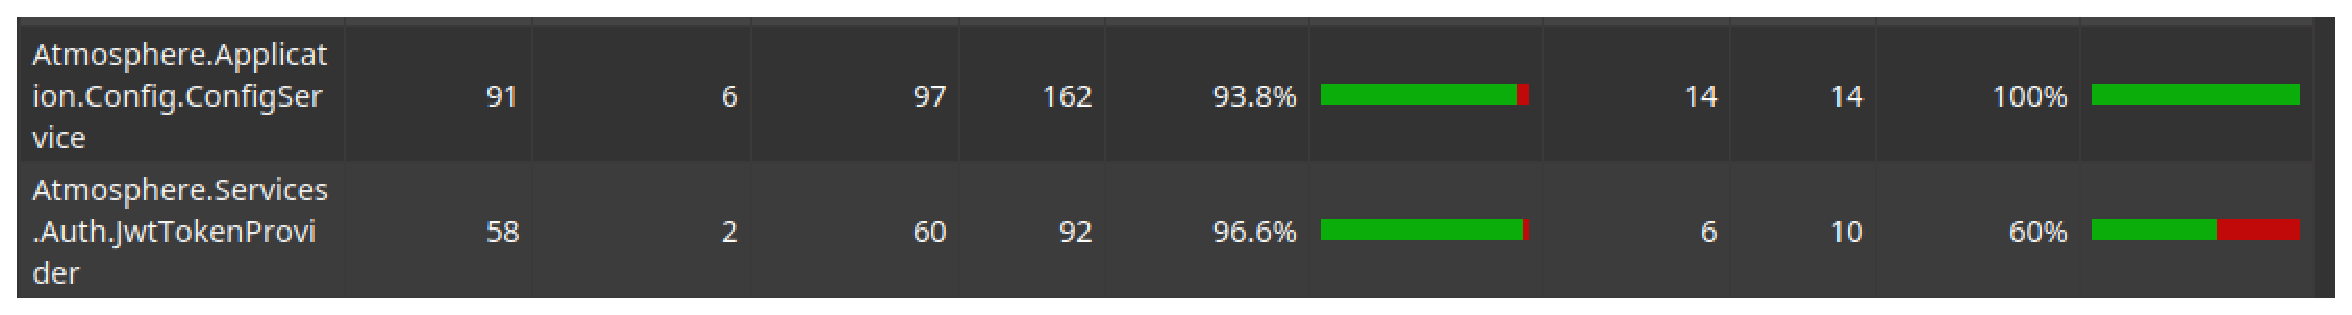
\includegraphics[width=\textwidth]{services_coverage}
  \caption{Procent linii pokrytych testami jednostkowymi w klasach \textbf{JwtTokenProvider} i \textbf{ConfigService}}
  \label{services:coverage}
\end{figure}
Warstwa zawierająca kontrolery nie wymagała testów - zawiera jedynie definicje punktów dostępu.
które wysyłają dalej zapytanie do warstwy aplikacyjnej poprzez wykorzystanie biblioteki MediatoR
oraz kod rejestrujący serwisy.
